\documentclass[12pt,a4paper,oneside]{book} %scrbook book report
\def\newblock{\hskip .11em plus .33em minus .07em}
\usepackage[english]{babel}
\usepackage{graphicx}
\graphicspath{figures/}
\usepackage{seecs}
\usepackage{url}
\usepackage{multirow}
\usepackage{amssymb,amsmath}
\usepackage{eucal}
\usepackage{nomencl}
\usepackage{natbib}
\usepackage{amsmath}
\usepackage[algoruled,vlined,linesnumbered,commentsnumbered,algochapter]{algorithm2e}
\usepackage{sfmath}

\setcounter{secnumdepth}{3}
\setcounter{tocdepth}{3}

\title{Web Based Overlay Network based on HTML5 \& JavaScript (WOvNet)}

\author{Umair Anwar}
\regno{2011-NUST-MS PhD-IT-19}
\degree{\MSIT}

\adviser{Dr. Ali Mustafa Qamar}
\adviserAffiliation{NUST-SEECS}

\date{{September 2013}}

\setcounter{tocdepth}{2}
%\linespread{1.1}

\begin{document}
\maketitle

\evaluationcommitteeapproval{Dr. Hammad Qureshi}{Dr. M. Usman Ilyas}{Mr. Bilal Ali}

\chapter*{Abstract}

Abstract Here

%---------------------------------------------------------------------
\certificateoforiginality
%---------------------------------------------------------------------
\chapter*{Acknowledgment}
Up and above everything all glory to {\bfseries ALMIGHTY ALLAH}. The Beneficent, The most Merciful and Most Compassionate. It's a great blessing from Almighty Allah that gives me the health and strength to do this research work.\\

I would like to special thank the {\bfseries Supervisor} .... and .....................\\

\begin{flushright} \textbf{Maqbool Ali} \end{flushright}
%---------------------------------------------------------------------

\tableofcontents
%
%\printnomenclature{2.5cm}
%\nomenclature{DCF}{Distributed Coordination Function}
%
%
\chapter*{List of Abbreviations}

\begin{table}[h]
   % increase table row spacing, adjust to taste
    \renewcommand{\arraystretch}{1.3}
    \label{table:table1}
     \begin{tabular}{ll}
        \hline\hline
        % inserting double-line
            {\bfseries Abbreviations} & {\bfseries Descriptions} \\
            \hline                                      % inserts single-line
            MLP & Multi Layer Perceptron  \\
            RBF & Radial Basis Function \\
            ANN & Artificial Neural Network  \\
            \hline                          % inserts single-line
    \end{tabular}
\end{table}

\listoffigures
\listoftables

%% \lstlistoflistings
%
\resetpagenumbering
%---------------------------------------------------------------------

\chapter{INTRODUCTION}\label{c-intro}
%-----------------------------------------------

Introduction here .................

The rest of the chapter is organized as follows. In Section 1.1, the problem statement is stated. In Section 1.2, thesis contributions are stated. In Section 1.3, we conclude the chapter with an outline for the rest of the thesis.

\section{Problem Statement}

Description of problem here...............

A formal problem statement is given as:

".................................."

\section{Thesis Contribution}

Our research work contributes in .................. areas.

All contributions of ................. are summarizing as follows:

\begin{itemize}
\item
Finding 1.
\item
Finding 2.
\end{itemize}

\section{Thesis Organization}

The rest of the thesis is organized as follows: \\

Chapter 2 discusses the state of the art related to the current research, and reviews the relevant literature aimed at finding .......................... \\

In Chapter 3, the .................... are discussed and then proposed methodology is presented. \\

In Chapter 4, the results are given along with detailed discussions. \\

In Chapter 5, the conclusion and future work is presented.

\chapter{LITERATURE REVIEW}\label{c-work}

In this chapter, literature related to ................ is presented.

Related to the \cite{umair} research related to the regression models for predictions is concerned, Ali et al.~\cite{ali} discussed the application of linear regression for future prediction using {\it SPSS} (Statistical Package for the Social Sciences). They found the P-values, beta scores, $R^2$, mean and standard deviation parameters that helped to learn good models for future prediction.

These regressions were found using response variable $y$ and predictor variable $x$ as shown in equations~\ref{eq2.13}-\ref{eq2.16}.
%
\begin{equation}
  y  =  w_0 + w_1 * x \; \mbox{(Linear)}
  \label{eq2.13}
\end{equation}
%
\begin{equation}
  y = w_0 + w_1 * x + w_2 * x^2 \; \mbox{(Quadratic)}
  \label{eq2.14}
\end{equation}
%
\begin{equation}
  y = w_0 + w_1 * x + w_2 * x^2 + w_3 * x^3 \; \mbox{(Cubic)}
  \label{eq2.15}
\end{equation}
%
\begin{equation}
  y = w_0 * x^{w_1} \; \mbox{(Power)}
  \label{eq2.16}
\end{equation}
%
\noindent where $w_0$, $w_1$, $w_2$,and $w_3$ are regression coefficients.

\chapter{IMPLEMENTATION}\label{c-implement}
In this chapter, the methodology that is used for modeling is explained.

Methodology Here .............................

\chapter{RESULTS AND DISCUSSION}\label{c-results}

This chapter presents detailed results along with relevant discussions. In this chapter, Section 4.1 explains the .................... results with detailed discussions; while Section 4.2 explains the ........... results with detailed discussions.

\section{Section Heading Here}

This section presents the results of ................

\subsection{Sub-Section Heading Here}

In order to perform ................

we have found that the pH is high in June and November as shown in Fig.~\ref{fig:Fig4}.  Fig.~\ref{fig:Fig4} shows........ Moreover, the trends for the remaining parameters are briefly described in Table~\ref{table:table13}.

\begin{figure}[!t]
  \centering
  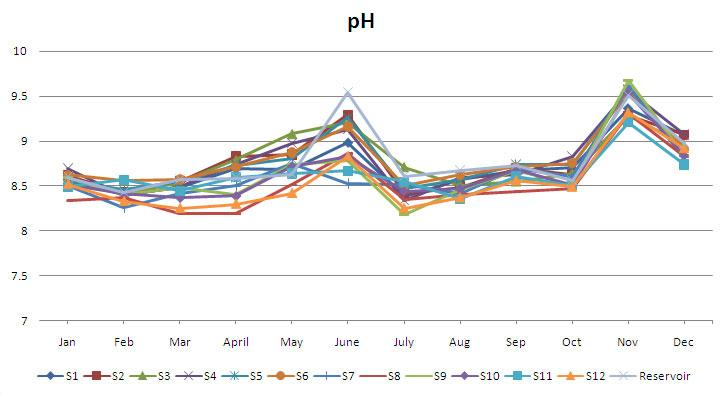
\includegraphics[width=3.25 in]{Fig-1.jpg}
  \caption{Month-wise pH Trend of Streams}
  \label{fig:Fig4}
\end{figure}

\begin{table}[!t]
  \begin{center}\scriptsize
     % increase table row spacing, adjust to taste
      \renewcommand{\arraystretch}{1.3}
      \caption{Month-wise Parametric Trend}
      \label{table:table13}
      \begin{tabular}{ll}
          \hline\hline
          % inserting double-line
              {\bfseries Parameter} & {\bfseries Trend} \\
              \hline                                      % inserts single-line
              Alkalinity & High values in February as compared to other months\\
              \hline                          % inserts single-line
      \end{tabular}
  \end{center}
\end{table}

\chapter{CONCLUSION AND FUTURE WORK}\label{c-conclusion}

In this chapter, the conclusion with a summary of the research findings along with future directions is presented.

\section{Conclusion}
Conclusion Here.........

\section{Future Work}
In future, the ..............

\begin{thebibliography}{10}

\bibitem{umair}
M. Ali, H. Qureshi, and M. S. Akhtar (2013), \emph{Analysis of growth in Students Intake and Degree Awarding Contribution: A Comparison of Stanford and MIT}, MLDM 2013: International Conference on Machine Learning and Data Mining, in press.

\end{thebibliography}

\end{document} 